%! Author = admin
%! Date = 2023/12/4

% Preamble
\documentclass[a4paper]{article}

% Packages
\usepackage[margin=1in]{geometry}
\usepackage[fontset=founder]{ctex}
\usepackage{anyfontsize}
\usepackage{graphicx}
\usepackage{amsmath}
\usepackage{amssymb}
\usepackage{mathabx}
\usepackage{multirow}
\usepackage{subfig}

\graphicspath{{../figures/}}

\title{\textbf{晶体管共射极单管放大器}}
\author{姚苏航\qquad PB22061220 \\ 庞宇乐\qquad PB22061166}
\date{实验时间: 2023年11月29日\qquad 座位号: 05}

% Document
\begin{document}
    \maketitle


    \section{实验目的\cite{ed4}}\label{sec:}

    \noindent{1.掌握放大器静态工作点的测量与调试方法。}

    \noindent{2.学习放大电路的交流特性等性能指标的测量方法。}

    \noindent{3.掌握静态工作点与输出波形失真的关系,了解最大不失真输出电压的测量方法。}
    \vspace{1cm}


    \section{实验原理}\label{sec:10}
    \begin{center}
        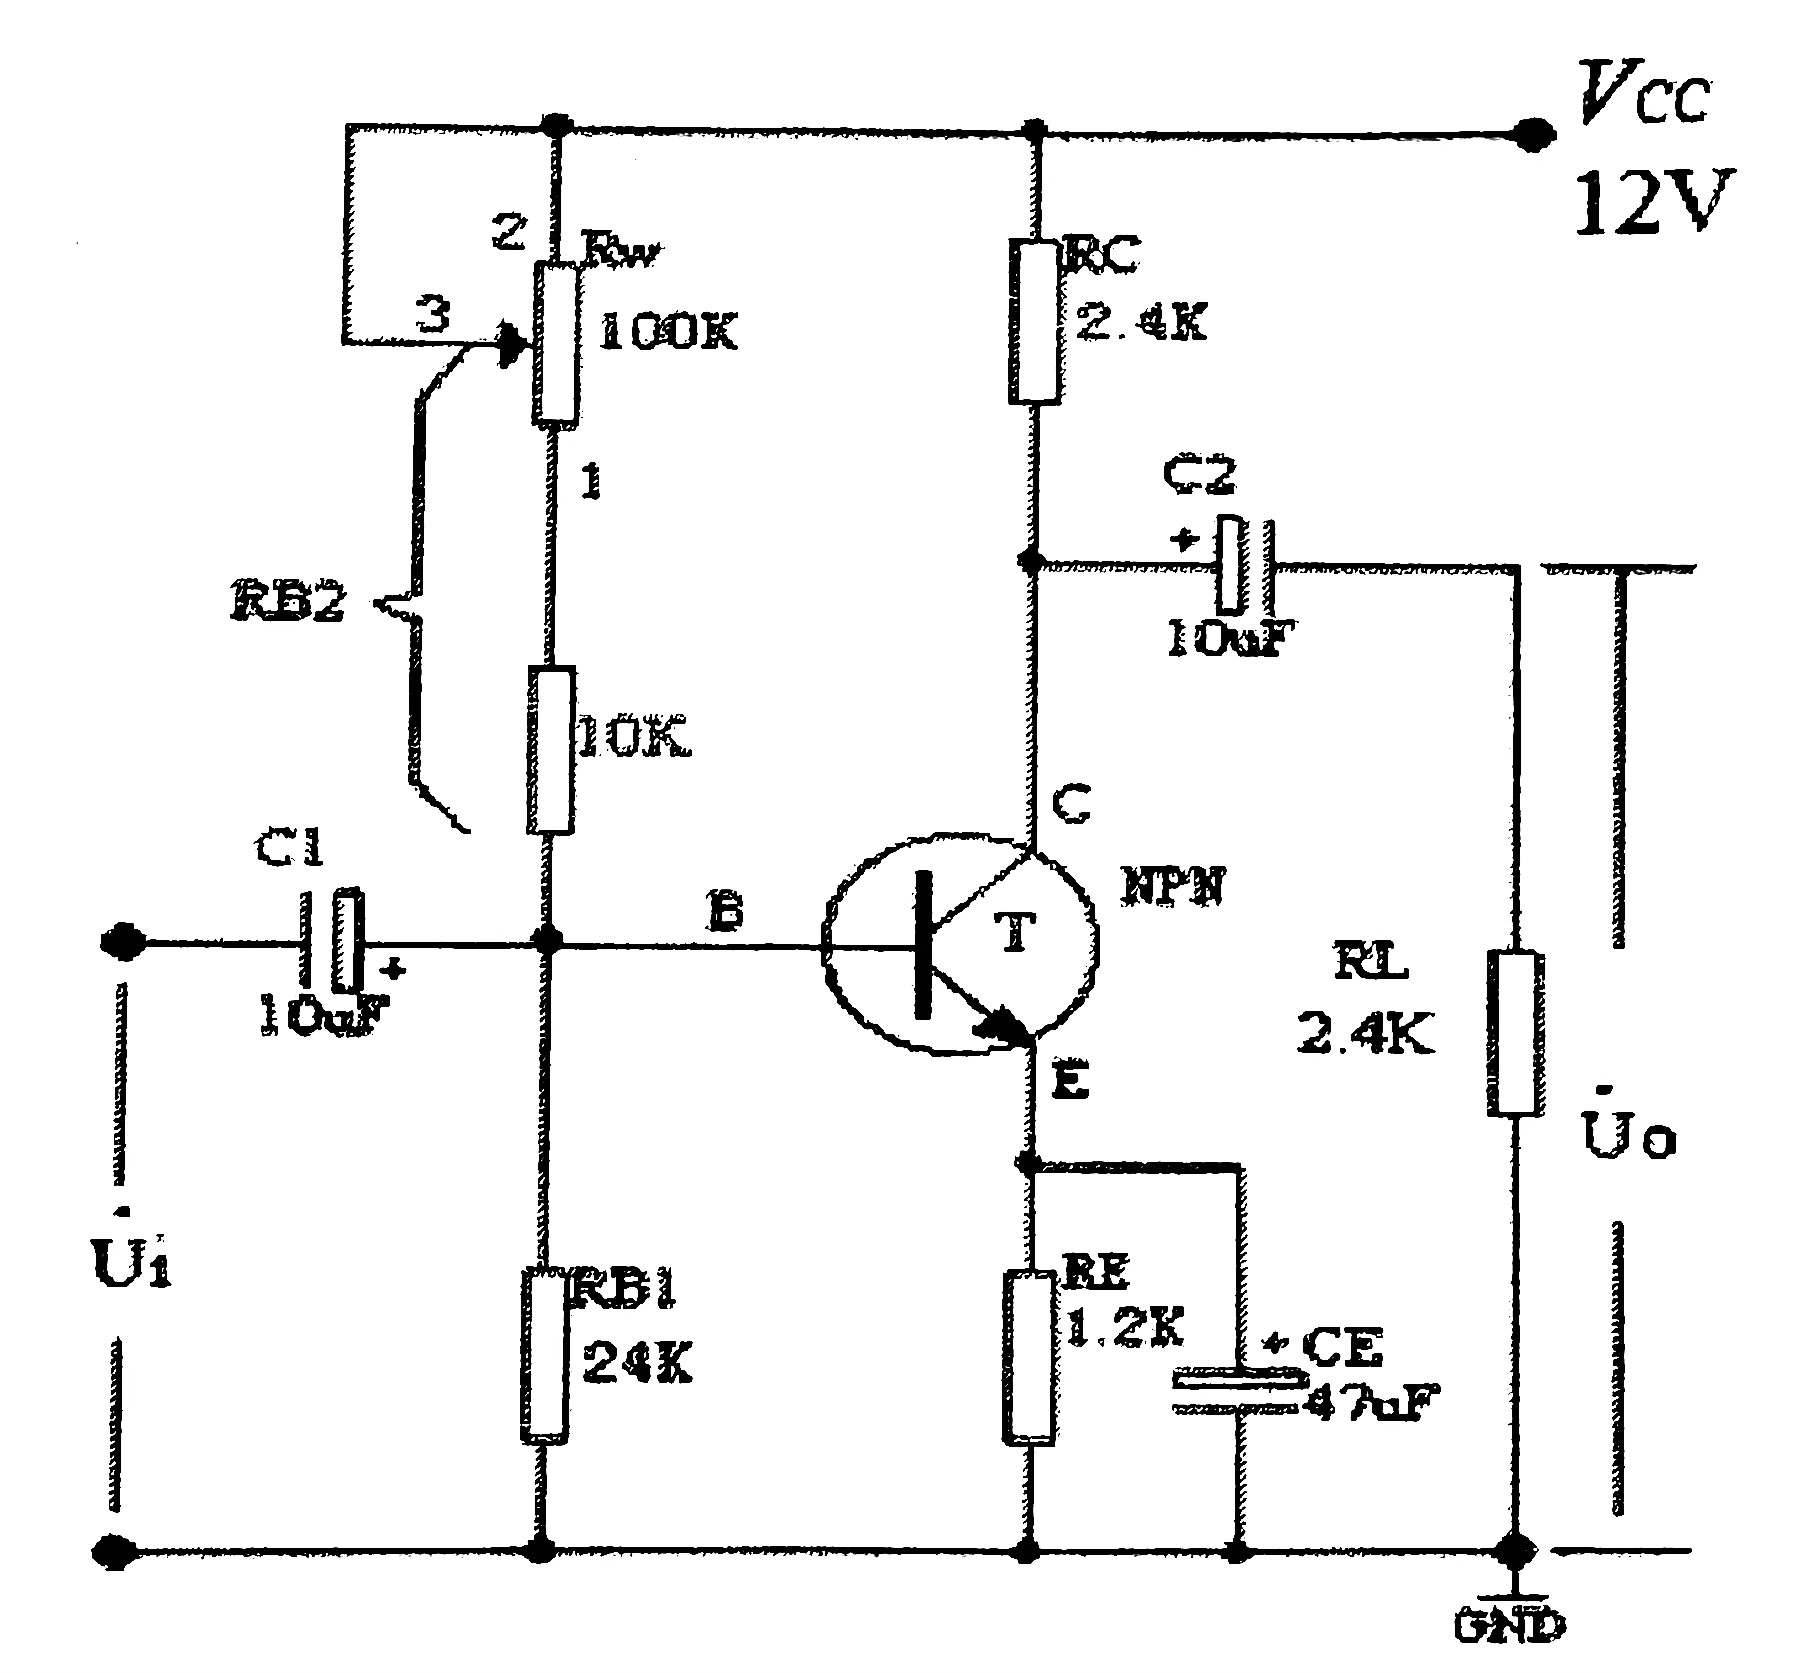
\includegraphics[height=170pt]{AC}\\
        {\small 图一:共射极单管放大电路}
    \end{center}

    {{图一为电阻分压式工作点稳定单管放大器实验电路图。
    其中偏置电路采用$R_{B1}$和$R_{B2}$组成的分压电路。
    $V_{CC}$作为集电极电源为电路提供能量,保证发射结正偏、集电结反偏。
    集电极电阻$R_C$将变化的电流转变成变化的电压,是电路具有电压放大能力。
    发射极电阻$R_E$引入负反馈稳定电路,稳定放大器静态工作点。
    耦合电容$C_1$和$C_2$隔离输入输出与电流直流的联系,同时能使信号顺利输入输出。}}
    \vspace{1cm}


    \section{实验仪器}\label{sec:2}
    \noindent{交流毫伏表,数字万用表,示波器,电路元件箱,信号发生器}
    \vspace{1cm}


    \section{测量静态工作点}\label{sec:3}

    \subsection{实验原理}\label{subsec:2}
    \begin{center}
        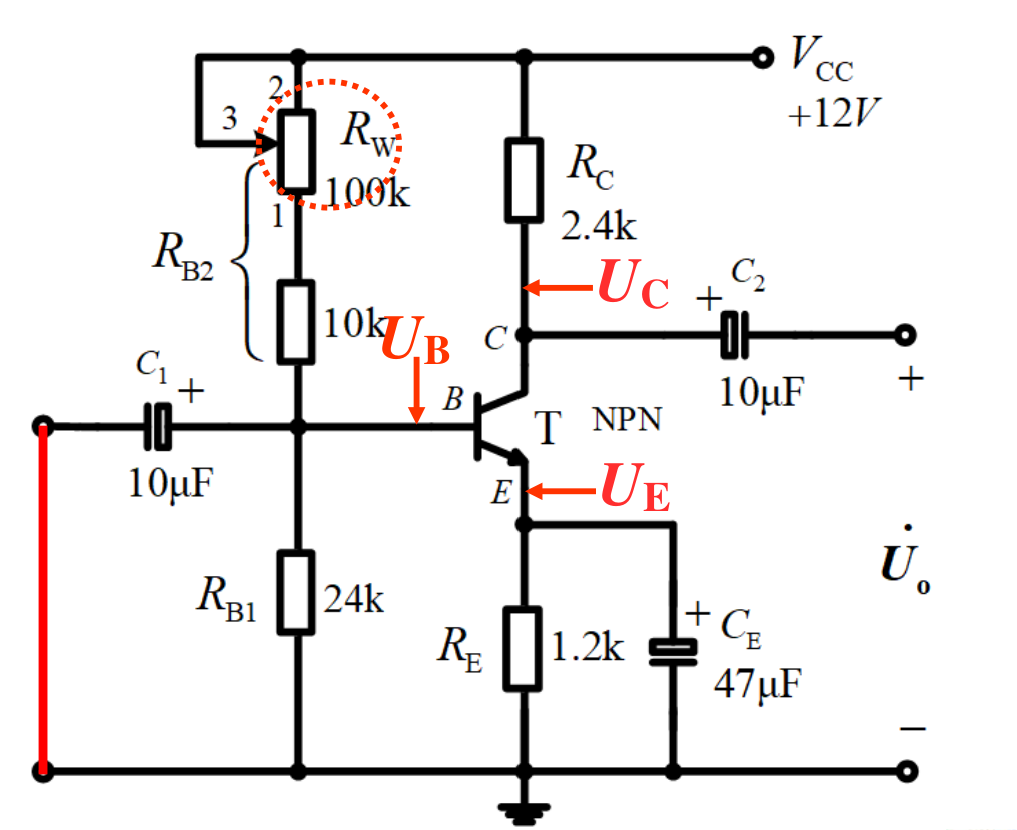
\includegraphics[height=170pt]{exp2}\\
        {\small 图二:实验电路}
    \end{center}

    {{测量放大器的静态工作点,应在输入信号$U_i=0$的情况下进行,
    即将放大器输入端与地端短接,然后选用量程合适的数字万用表,
    分别测量晶体管的集电极电流$I_c$以及各电极对地的电位$U_B$、$U_C$和$U_E$。}}

    {{一般实验中,为了避免断开集电极,所以采用测量电压,然后算出$I_C$的方法。
    例如,只要测出$U_E$,即可求出$I_C$}}

    \begin{equation}
        I_C\approx I_E=\frac{U_E}{R_E}\label{eq:equation}
    \end{equation}

    {{也可根据下式得到:}}

    \begin{equation}
        \begin{aligned}
            I_C&=\frac{V_{CC}-U_C}{R_C}\\
            U_{BE}&=U_B-U_E\\
            U_{CE}&=U_C-U_E\label{eq:equation2}
        \end{aligned}
    \end{equation}

    \subsection{实验内容}\label{subsec:}
    {{按照图一中的电路接线,打开交流开关,调节$R_W$,
    使$I_C=2.0mA$(即$U_E=2.4V$),
    用万用表测量$U_B$、$U_C$、$U_E$和$R_{B2}$。}}

    \subsection{实验数据}\label{subsec:3}
    {{实验数据记录如下表所示:}}

    \begin{table}[htbp]
        \centering
        \caption{静态工作点测量数据}
        \begin{tabular}{|c|c|c|c|c|c|c|}
            \hline
            \multicolumn{4}{|c|}{测量值} & \multicolumn{3}{|c|}{计算值} \\
            \hline
            $U_B(V)$ & $U_E(V)$ & $U_C(V)$ & $R_{B2}(k\Omega)$ & $U_{BE}(V)$ & $U_{CE}(V)$ & $I_C(mA)$ \\
            \hline
            3.008    & 2.403    & 7.147    & 65.42k            & 0.605       & 4.744       & 2.003     \\
            \hline
        \end{tabular}\label{tab:table2}
    \end{table}

    \subsection{注意事项}\label{subsec:4}
    {{静态工作点的测量条件:输入接地(即$U_i=0$)。}}
    {{在记录电位器$R_W$值时,要使$R_W$与电路断开,没有电流流过。}}
    \vspace{1cm}


    \section{测量电压放大倍数}\label{sec:4}

    \subsection{实验原理}\label{subsec:5}
    {{调节放大器到静态工作点时,然后加入输入电压$u_i$,在输出电压$u_o$不失真的情况下,
    用交流毫伏表或者示波器测出$u_i$和$u_o$的有效值$U_i$和$U_o$,则}}

    \begin{equation}
        A_u=\frac{U_o}{U_i}\label{eq:equation3}
    \end{equation}

    \subsection{实验内容}\label{subsec:6}
    {{调节频率为$1kHz$的正弦波作为输入信号$u_i$。
    同时用双踪示波器观察放大器输入电压$u_i$和输出电压$u_o$的波形,
    在$u_o$波形不失真的条件下,用毫伏表或者示波器测量开路和带载两种情况下$u_o$的有效值,
    并用双踪示波器观察$u_o$和$u_i$的相位关系。}}

    \subsection{实验数据}\label{subsec:7}
    {{记录实验数据如下表:}}
    \begin{table}[htbp]
        \centering
        \caption{$I_c=2.0mA\quad U_i=10mV$(有效值)}
        \begin{tabular}{|c|c|c|c|}
            \hline
            $R_C(k\Omega)$ & $R_L(k\Omega)$ & $U_o(V)$ & $A_u$ \\
            \hline
            2.4            & 2.4            & 0.675    & 67.5  \\
            \hline
            2.4            & $\infty$       & 1.359    & 135.9 \\
            \hline
        \end{tabular}\label{tab:table3}
    \end{table}

    {{观察记录的$u_o$和$u_i$波形如图三所示:}}

    \begin{center}
        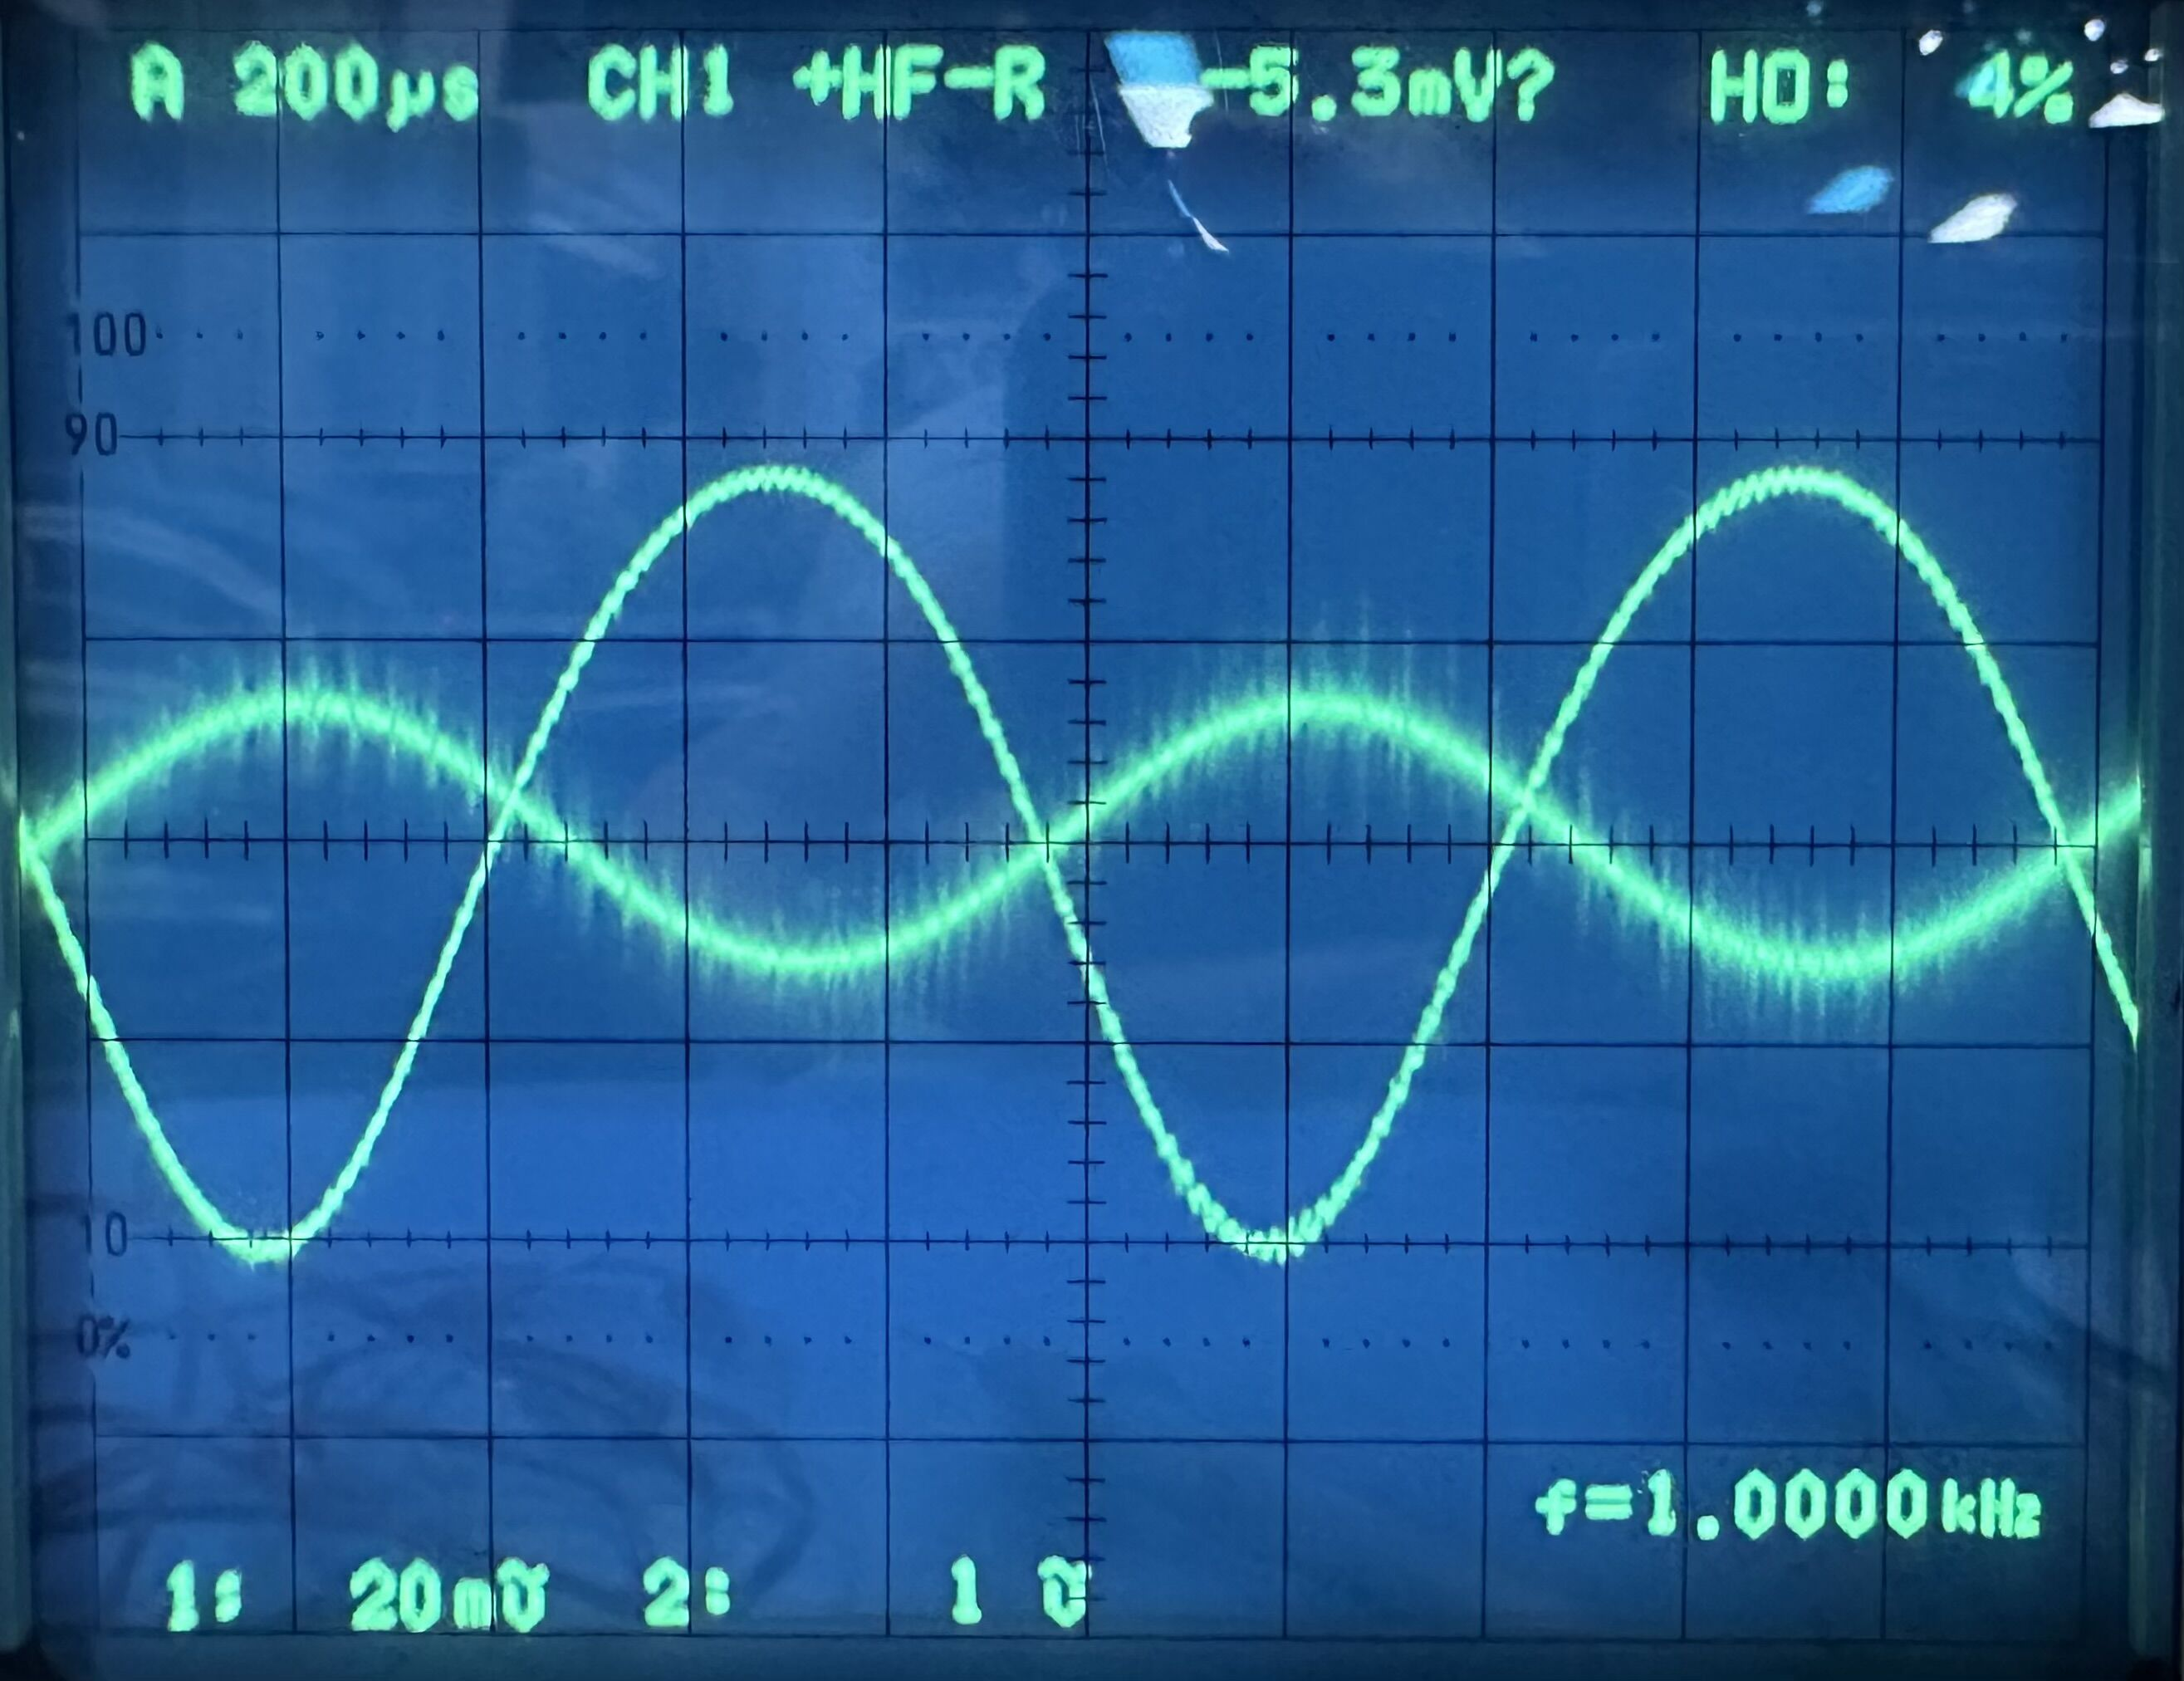
\includegraphics[height=130pt]{ref}\\
        {\small 图三:$u_o$和$u_i$的相位关系}
    \end{center}

    \subsection{注意事项}\label{subsec:8}
    {{在测试$f_H$与$f_L$过程中要保持输入电压$U_i$不变。}}
    {{当频率较高时,示波器已不是理想的测量设备,要把示波器从放大电路的输出端断开。}}
    \vspace{1cm}


    \section{测量输入电阻和输出电阻}\label{sec:5}

    \subsection{实验原理}\label{subsec:9}
    {{输入电阻:串联电阻法。在输入回路串联取样电阻$R$,
    直接测量取样电阻$R$两端的信号电压:$U_s$、$U_i$。
    根据输入电阻的定义可得:}}

    \begin{equation}
        R_i=\frac{U_i}{I_i}=\frac{U_i}{U_s-U_i}R\label{eq:equation4}
    \end{equation}

    {{输出电阻:两次电压法。先测量开路电压$U_o$,再测量接入负载后的输出电压$U_L$,则:}}
    \begin{equation}
        R_o=(\frac{U_o}{U_L}-1)R_L\label{eq:equation5}
    \end{equation}

    \subsection{实验内容}\label{subsec:10}
    \begin{center}
        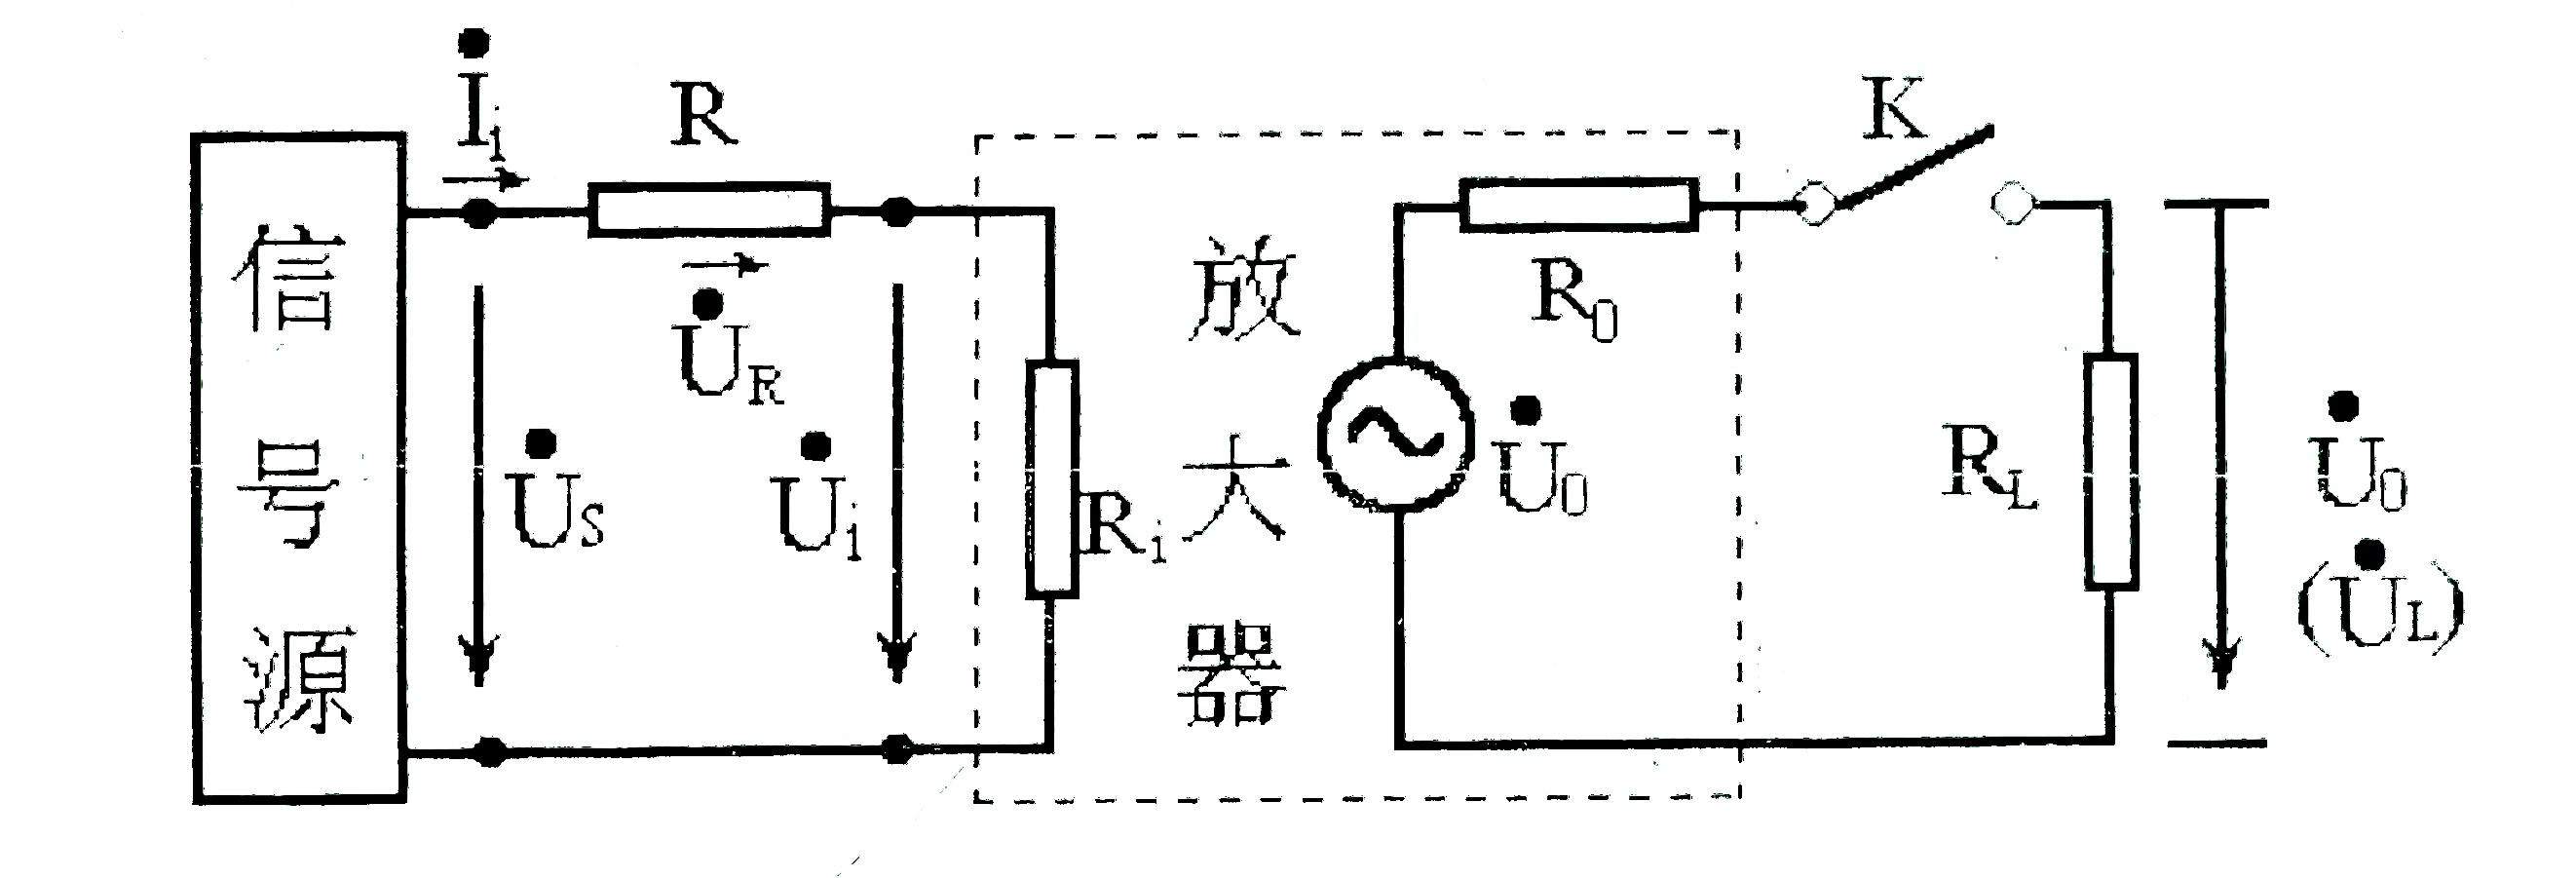
\includegraphics[height=125pt]{R}\\
        {\small 图四:实验电路}
    \end{center}

    {{按图四接线,取$R=2k\Omega$,置$R_C=2.4k\Omega$、$R_L=2.4k\Omega$、$I_C=2.0mA$。
    输入$f=1kHz$的正弦信号$u_s$,在输出电压$u_o$不失真的条件下,
    用毫伏表或者示波器测量$U_s$、$U_i$,根据公式\eqref{eq:equation4}求出$R_i$。}}
    {{输出电阻$R_o$可根据公式\eqref{eq:equation5}求出。}}

    \subsection{实验数据与误差分析}\label{subsec:11}

    \subsection{注意事项}\label{subsec:12}
    {{必须保持$R_L$接入电路前后输入信号的大小不变。}}
    {{在测量$U_s$和$U_i$电压值时,为了减小测量误差,只能用毫伏表的同一路做测试。}}
    \vspace{1cm}


    \section{测量幅频特性曲线}\label{sec:6}

    \subsection{实验原理}\label{subsec:13}
    {{随着信号频率的变化,当电压放大倍数下降到中频放大倍数的$\frac{1}{\sqrt{2}}$倍即$0.707A_{um}$时,
    其所对应的频率分别称为下截止频率$f_L$和上截止频率$f_H$,如图五所示,
    则$f_L$与$f_H$之间的范围就称为放大电路的通频带$BW$。}}
    \begin{center}
        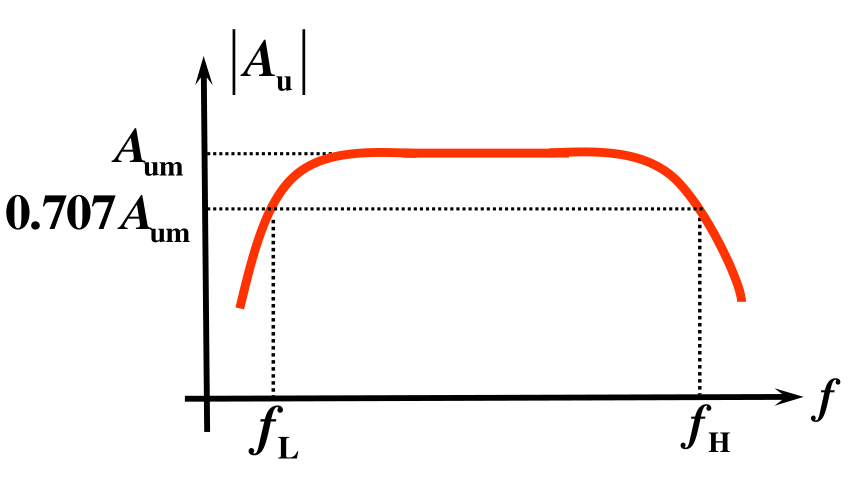
\includegraphics[height=130pt]{Af}\\
        {\small 图五:理想幅频特性曲线}
    \end{center}

    \subsection{实验内容}\label{subsec:14}
    {{取$IC=2.0mA$,$RC=2.4k\Omega$,$RL=2.4k\Omega$。
    保持输入信号$u_i$不变,改变信号源频率$f$,逐点测出相应的输出电压$U_o$,
    自作表格并记录之。}}

    \subsection{实验数据}\label{subsec:15}
    {{实验数据记录如下表所示:}}
    \begin{table}[htbp]
        \centering
        \caption{测量数据}
        \begin{tabular*}{\textwidth}{@{\extracolsep{\fill}}|l|l|l|l|l|l|l|l|}
            \hline
            f/Hz     & 200    & 250    & 269    & 270    & 271     & 280    & 300    \\
            \hline
            $U_o$/V  & 0.442  & 0.492  & 0.512  & 0.513  & 0.514   & 0.52   & 0.534  \\
            \hline
            $U_i$/mV & 9.30   & 9.30   & 9.30   & 9.30   & 9.29    & 9.29   & 9.28   \\
            \hline
            |Au|     & 47.527 & 52.903 & 55.054 & 55.161 & 55.3281 & 55.974 & 57.543 \\
            \hline
        \end{tabular*}

        \begin{tabular*}{\textwidth}{@{\extracolsep{\fill}}|l|l|l|l|l|l|l|l|}
            \hline
            f/Hz     & 500    & 1000   & 3000   & 5000   & 10000  & 15000  & 20000  \\
            \hline
            $U_o$/V  & 0.619  & 0.678  & 0.709  & 0.713  & 0.717  & 0.717  & 0.717  \\
            \hline
            $U_i$/mV & 9.27   & 9.24   & 9.22   & 9.21   & 9.19   & 9.18   & 9.18   \\
            \hline
            |Au|     & 66.774 & 73.377 & 76.898 & 77.416 & 78.020 & 78.104 & 78.104 \\
            \hline
        \end{tabular*}

        \begin{tabular*}{\textwidth}{@{\extracolsep{\fill}}|l|l|l|l|l|l|l|l|}
            \hline
            f/Hz     & 30000  & 70000  & 100000 & 200000 & 300000 & 400000 & 470000 \\
            \hline
            $U_o$/V  & 0.716  & 0.705  & 0.693  & 0.638  & 0.568  & 0.498  & 0.459  \\
            \hline
            $U_i$/mV & 9.16   & 9.13   & 9.10   & 8.91   & 8.69   & 8.45   & 8.28   \\
            \hline
            |Au|     & 78.166 & 77.218 & 76.154 & 71.605 & 65.362 & 58.935 & 55.435 \\
            \hline
        \end{tabular*}

        \begin{tabular*}{\textwidth}{@{\extracolsep{\fill}}|l|l|l|l|l|l|l|l|}
            \hline
            f/Hz     & 475000 & 480000 & 485000 & 490000 & 495000 & 500000 & 700000 \\
            \hline
            $U_o$/V  & 0.458  & 0.456  & 0.455  & 0.451  & 0.448  & 0.445  & 0.349  \\
            \hline
            $U_i$/mV & 8.27   & 8.26   & 8.25   & 8.24   & 8.23   & 8.22   & 7.87   \\
            \hline
            |Au|     & 55.381 & 55.206 & 55.152 & 54.733 & 54.435 & 54.136 & 44.346 \\
            \hline
        \end{tabular*}\label{tab:table}
    \end{table}

    {{根据上表中数据,用origin拟合图像得:}}
    \begin{center}
        \includegraphics[height=200pt]{Graph1}\\
        {\small 图六:实际幅频特性曲线}
    \end{center}

    \subsection{注意事项}\label{subsec:16}
    {{为使频率$f$取值合适,可以先粗测一下,找出中频范围,然后再仔细读数。}}
    \vspace{1cm}


    \section{观察静态工作点对输出波形失真的影响}\label{sec:7}

    \subsection{实验原理}\label{subsec:17}
    \begin{figure*}[htbp]
        \centering
        \subfloat[饱和失真与截止失真]{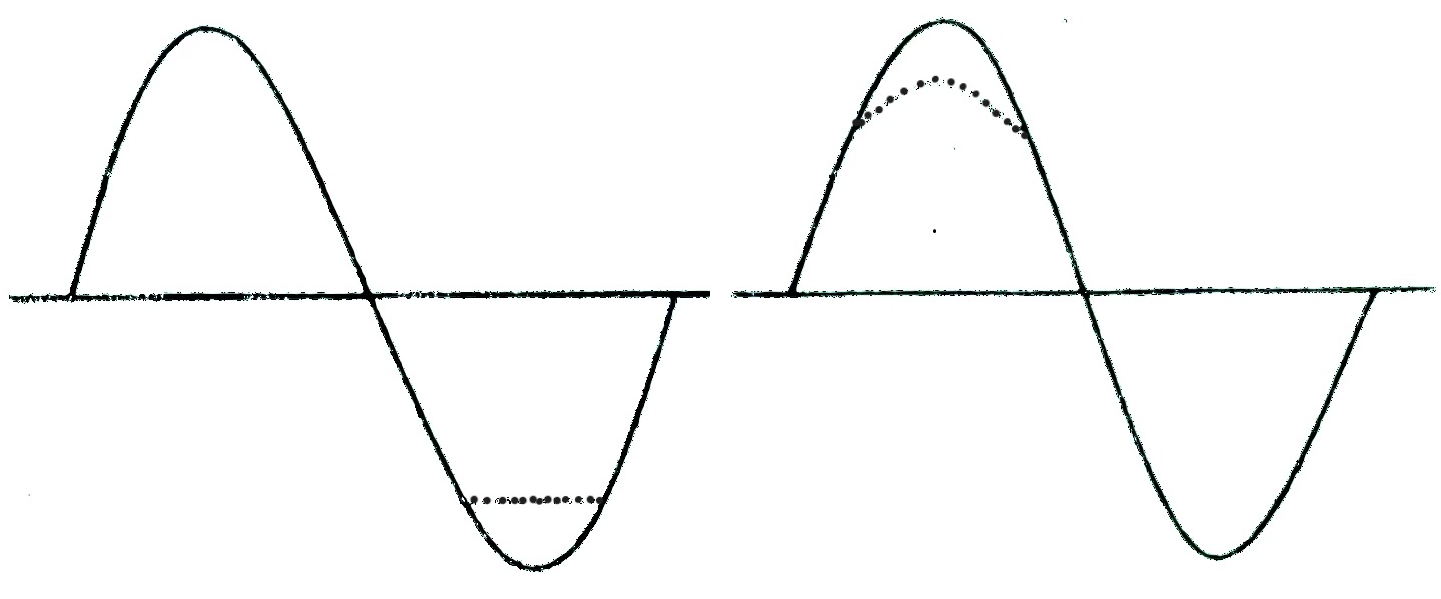
\includegraphics[height=100pt]{ID2}}
        \subfloat[电路参数对静态工作点影响]{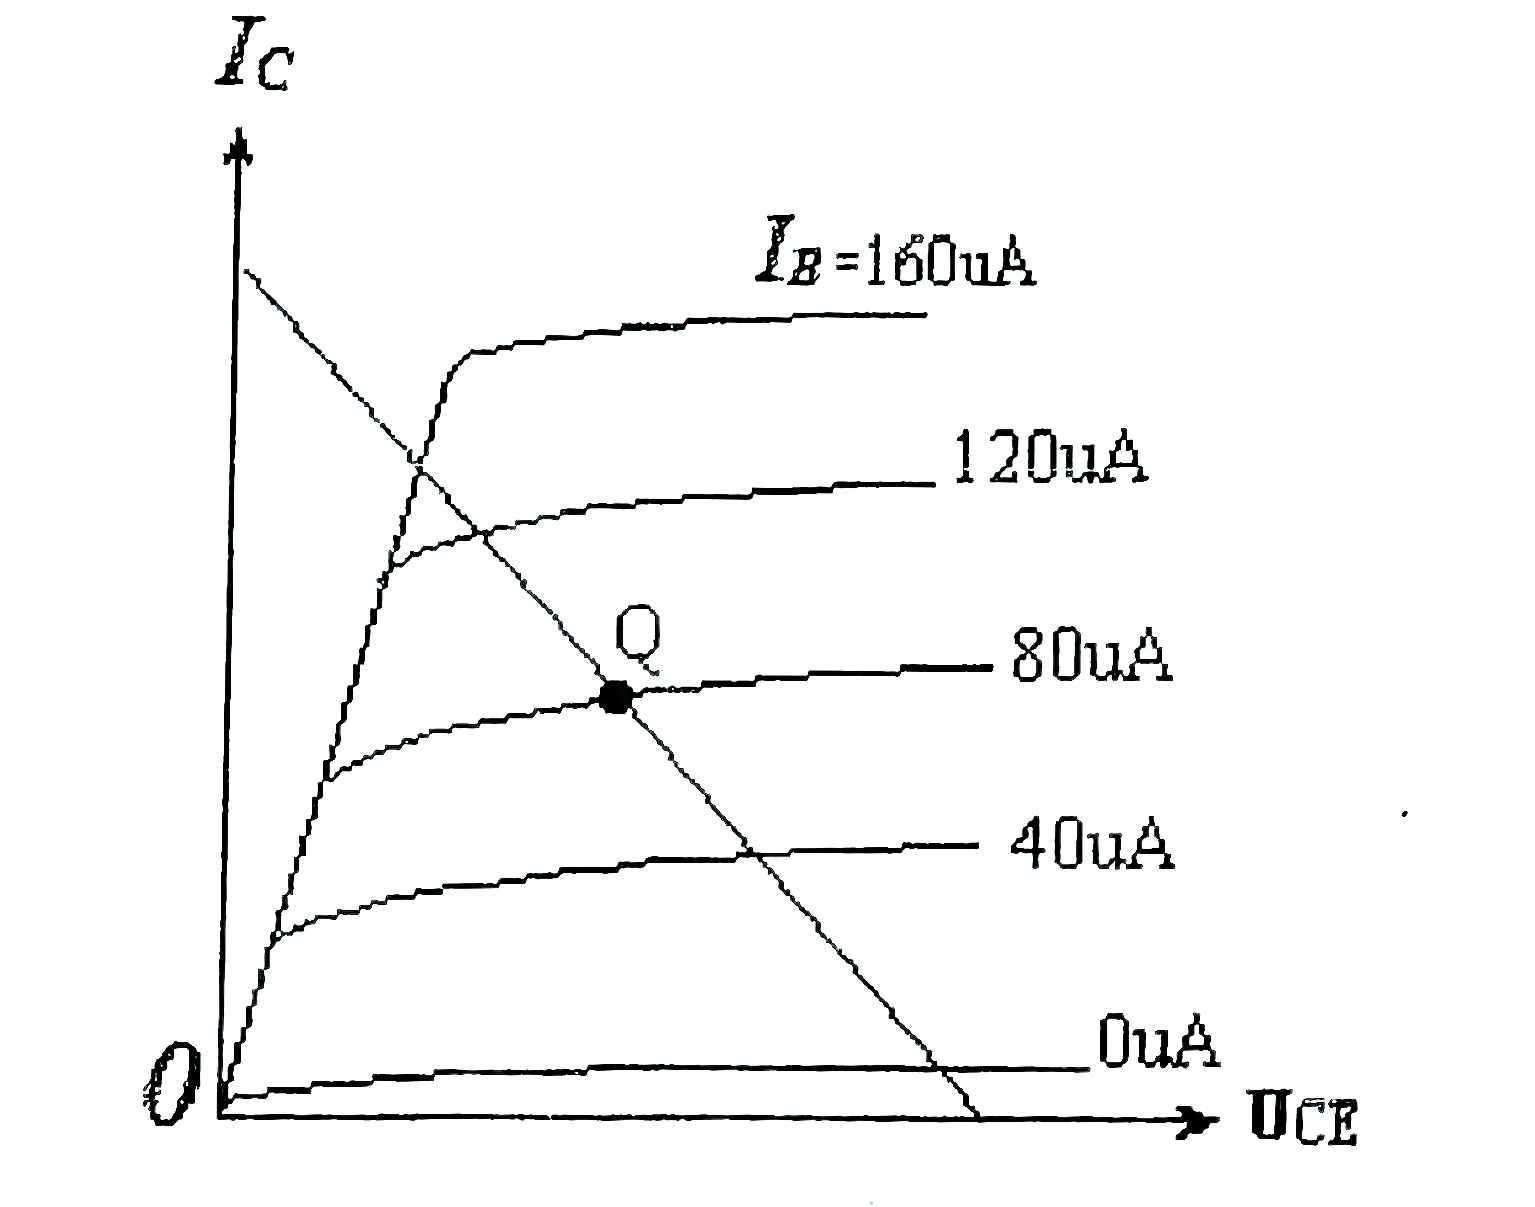
\includegraphics[height=100pt]{IU}}\\
        {\small 图七:理论图像}
    \end{figure*}
    {{$I_{CQ}\uparrow$,三极管进入饱和区而引起饱和失真,形状为“削底”失真。通过增大基极偏置电阻的阻值来消除。}}
    {{$I_{CQ}\downarrow$,三极管进入截止区而引起截止失真,形状为“缩顶”失真。通过减小基极偏置电阻的阻值来消除。}}
    {{$I_{CQ}$正常,即工作点选在交流负载线的中心,当加大输入信号时,$u_o$同时出现饱和与截止失真。}}

    \subsection{实验内容}\label{subsec:18}
    {{按图八接好实验电路,在$R_C=2.4k\Omega$、$R_L=+\infty$连线条件下,使$u_i=0$,调节$R_W$使$I_C=2.0mA$,测出$U_{CE}$值。
    输入频率为$1kHz$的正弦波信号$u_i$,再逐步加大输入信号幅度,使输出电压$u_o$足够大但不失真。
    然后保持输入信号不变,分别增大和减小$R_W$,使波形出现失真,绘出$u_o$的波形,并测出失真情况下的$I_C$和$U_{CE}$值,记录在表格中。}}
    \begin{center}
        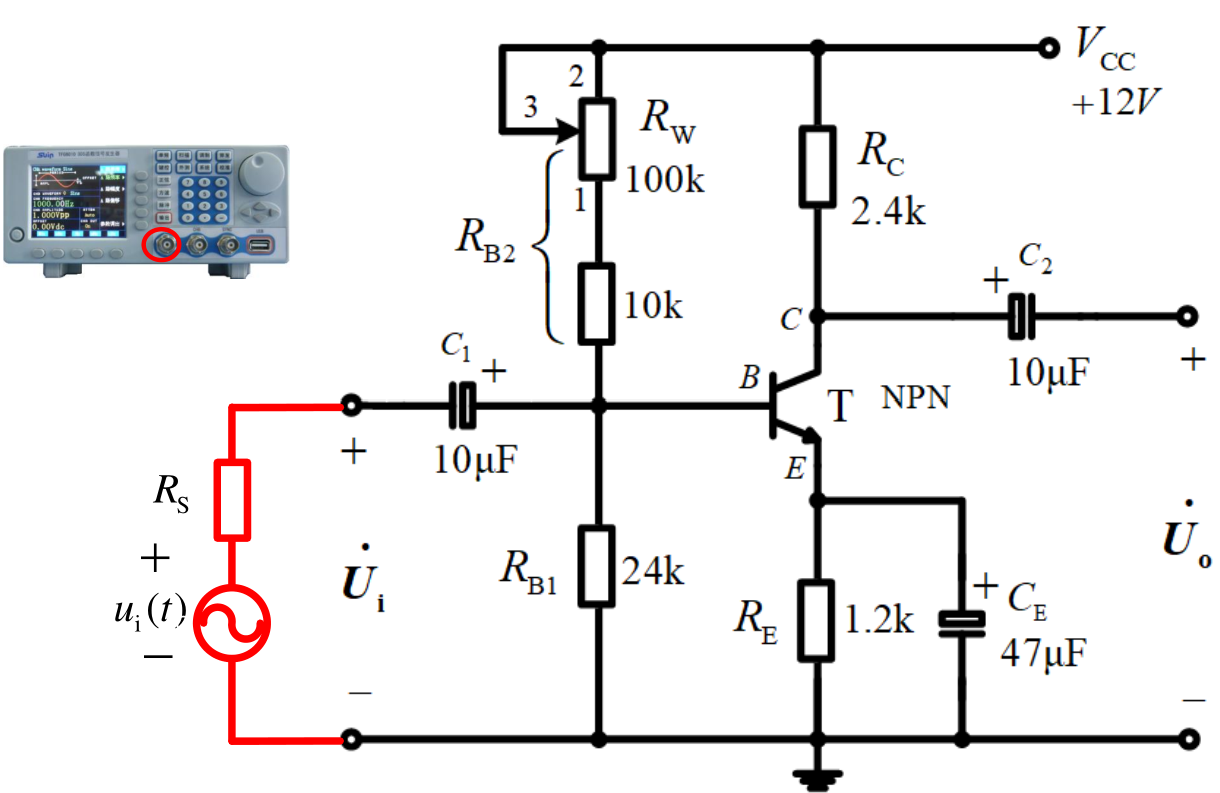
\includegraphics[height=150pt]{exp5}\\
        {\small 图八:实验电路}
    \end{center}

    \subsection{实验数据}\label{subsec:19}
    {{实验数据记录如下表所示:}}
    \begin{table}[htbp]
        \centering
        \caption{$R_C=2.4k\Omega\quad R_L=\infty\quad U_i=21mV$}
        \begin{tabular}{|c|c|c|c|c|c|}
            \hline
            $U_B(V)$ & $U_E(V)$ & $U_C(V)$ & $R_{B2}(\Omega)$ & 失真情况 & 管子工作状态 \\
            \hline
            2.039    & 1.531    & 9.031    & 107.95k          & 截止失真 & 截止区    \\
            \hline
            3.008    & 2.404    & 7.232    & 66.77k           & 不失真  & 放大区    \\
            \hline
            3.699    & 3.322    & 5.851    & 44.83k           & 饱和失真 & 饱和区    \\
            \hline
        \end{tabular}\label{tab:table4}
    \end{table}

    {{三种失真情况下的$u_o$波形如图九所示:}}
    \begin{figure*}[htb]
        \centering
        \subfloat[截止失真]{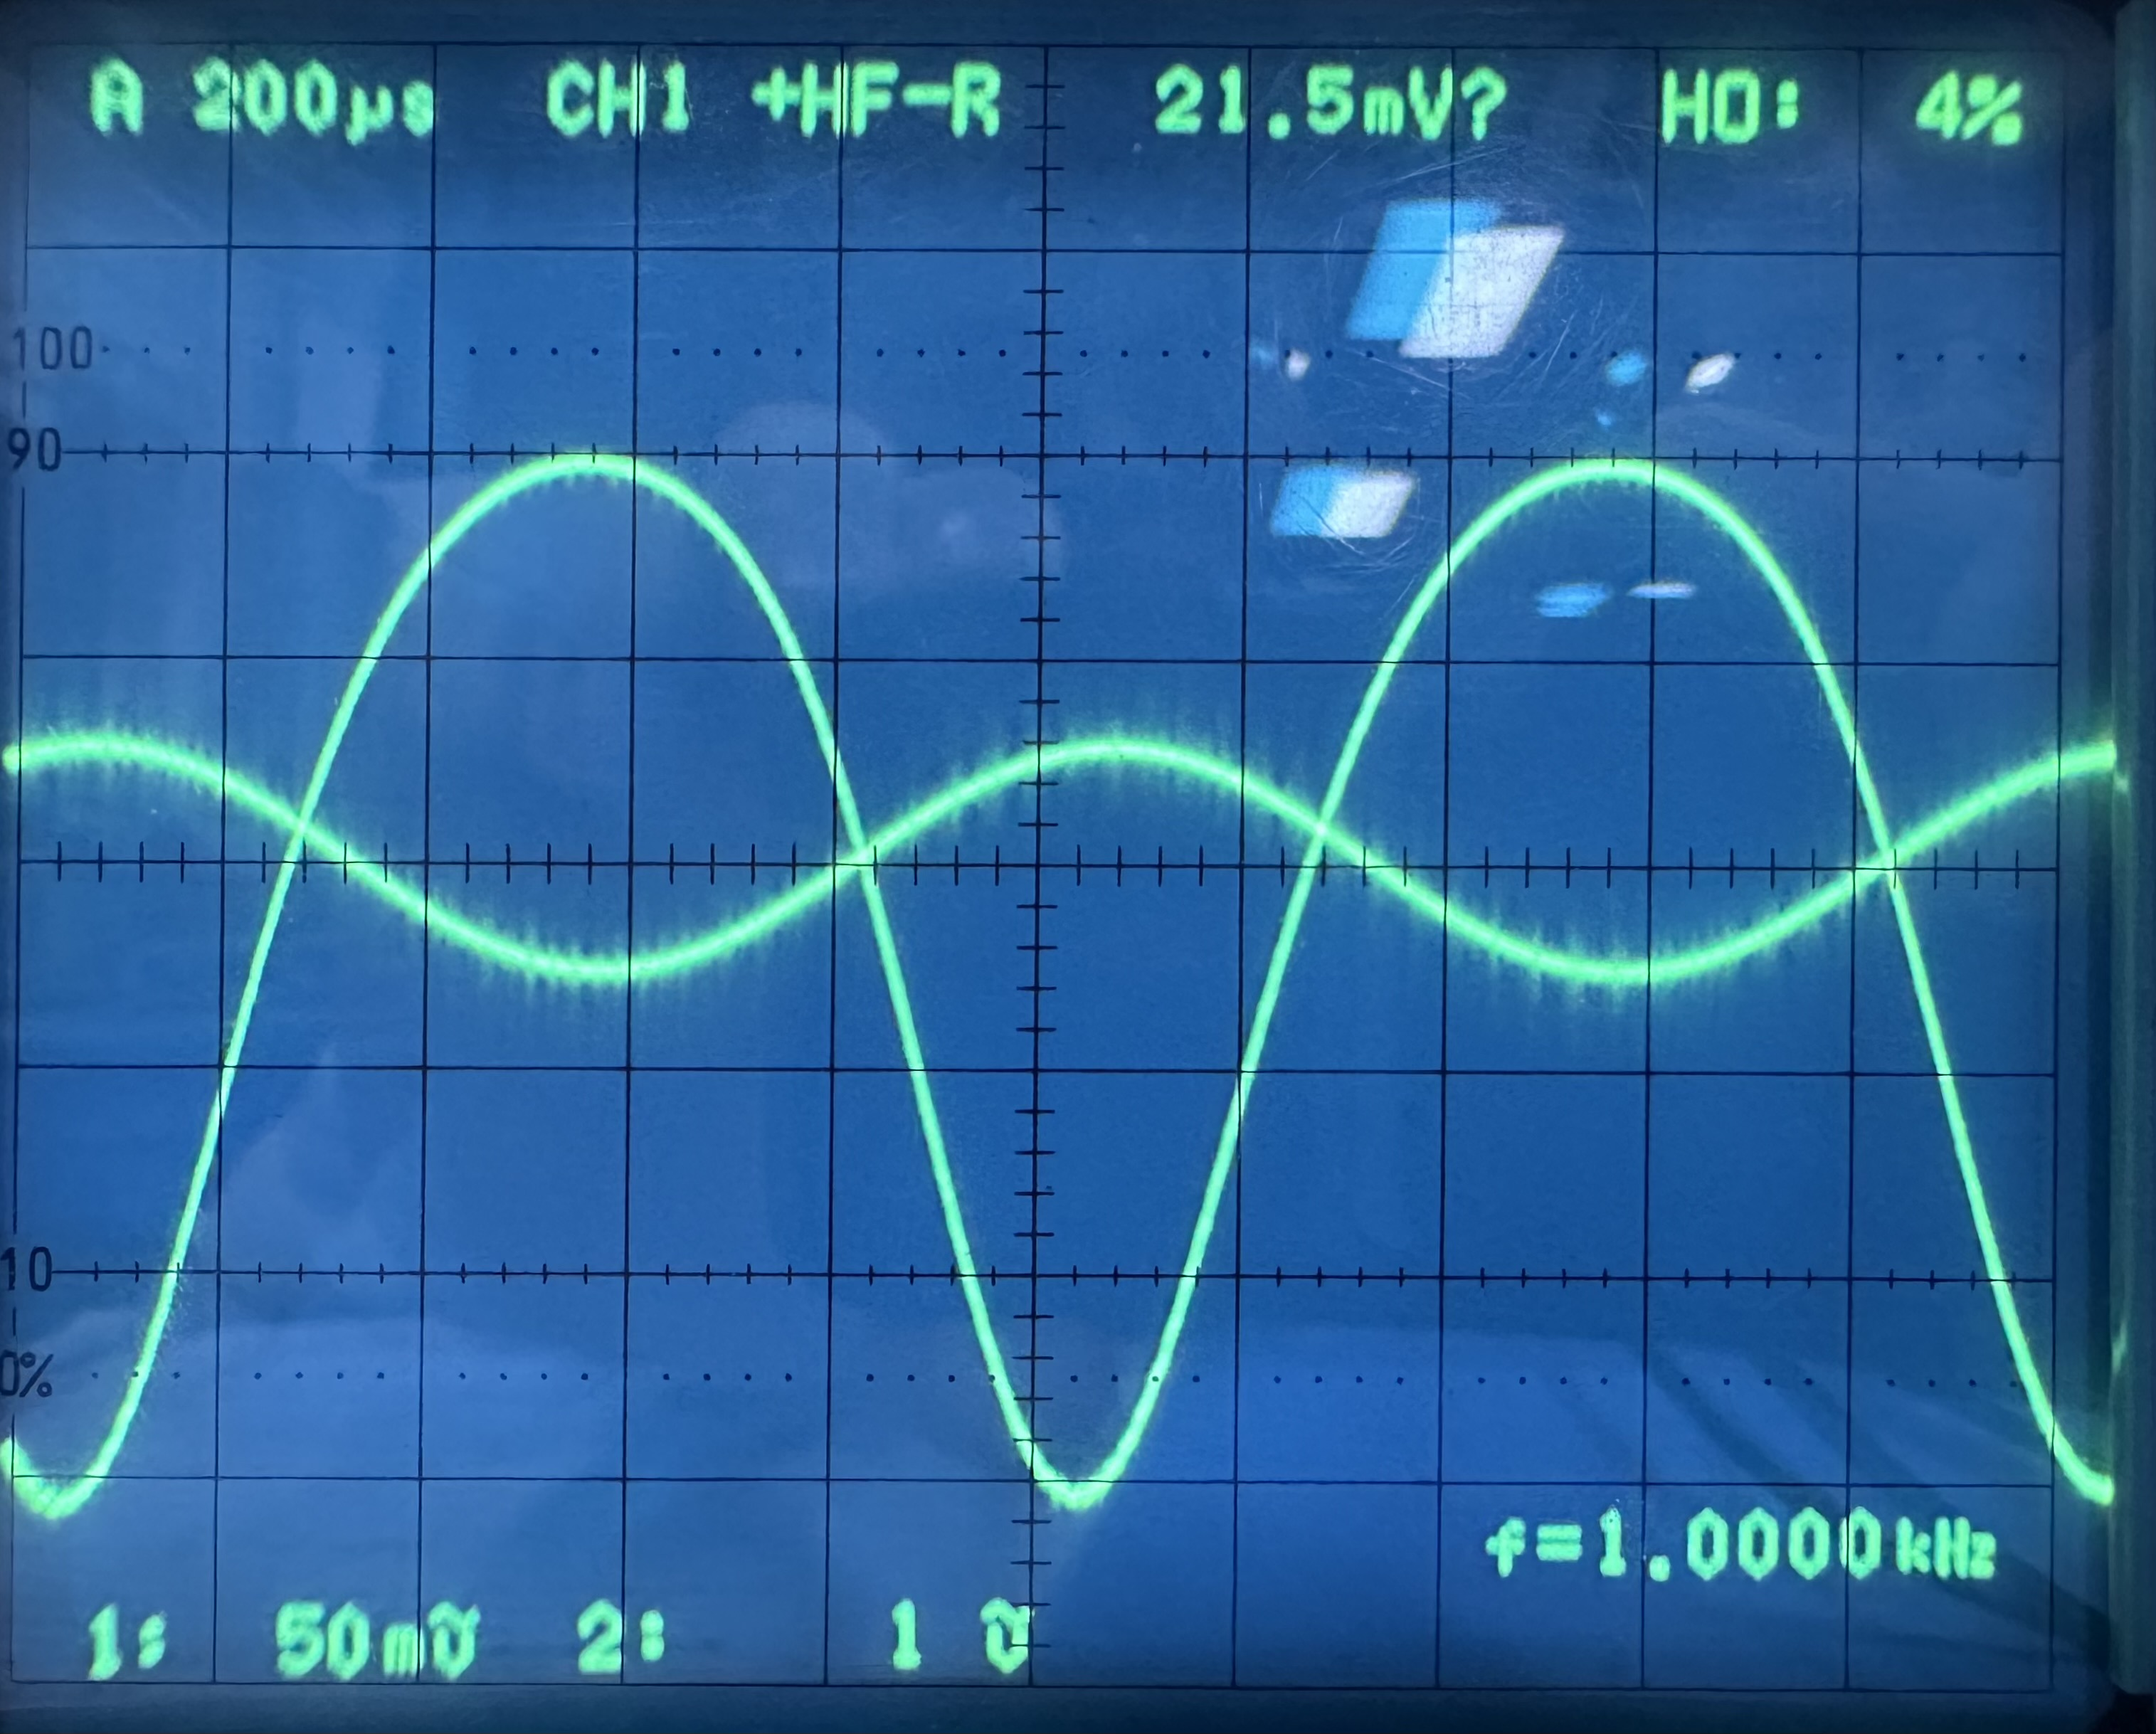
\includegraphics[height=110pt]{TD}}
        \subfloat[不失真]{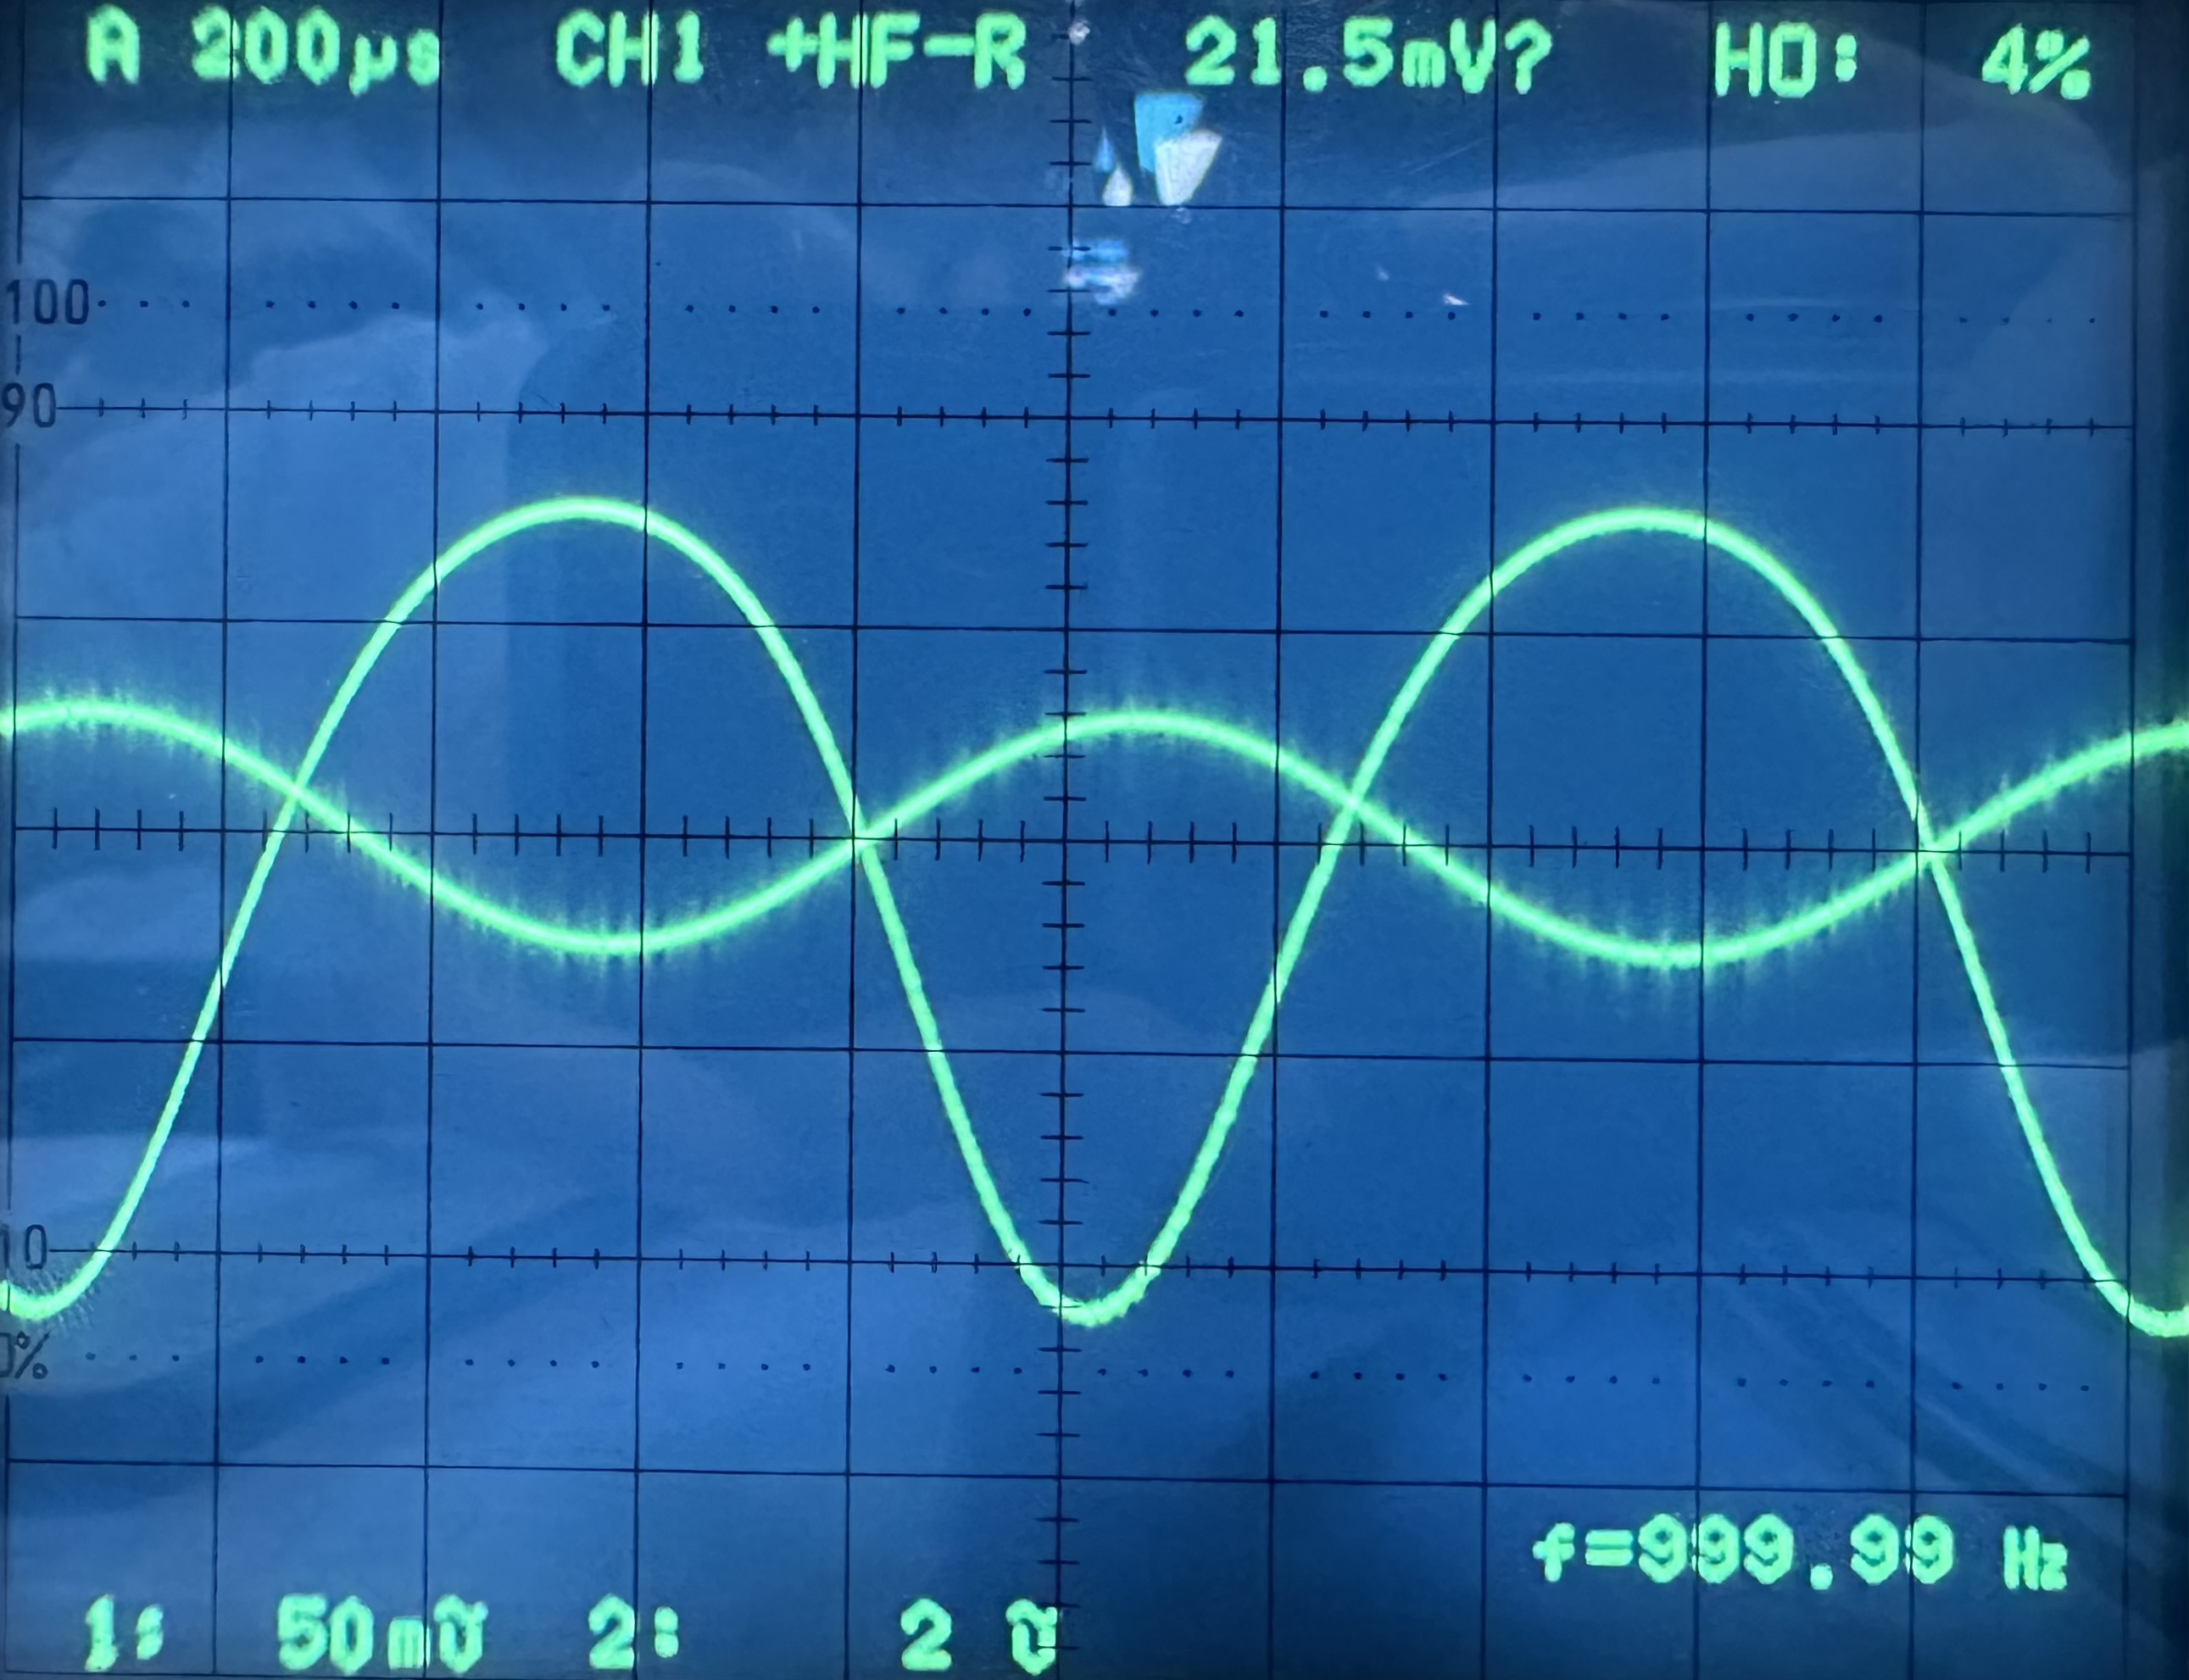
\includegraphics[height=110pt]{O}}
        \subfloat[饱和失真]{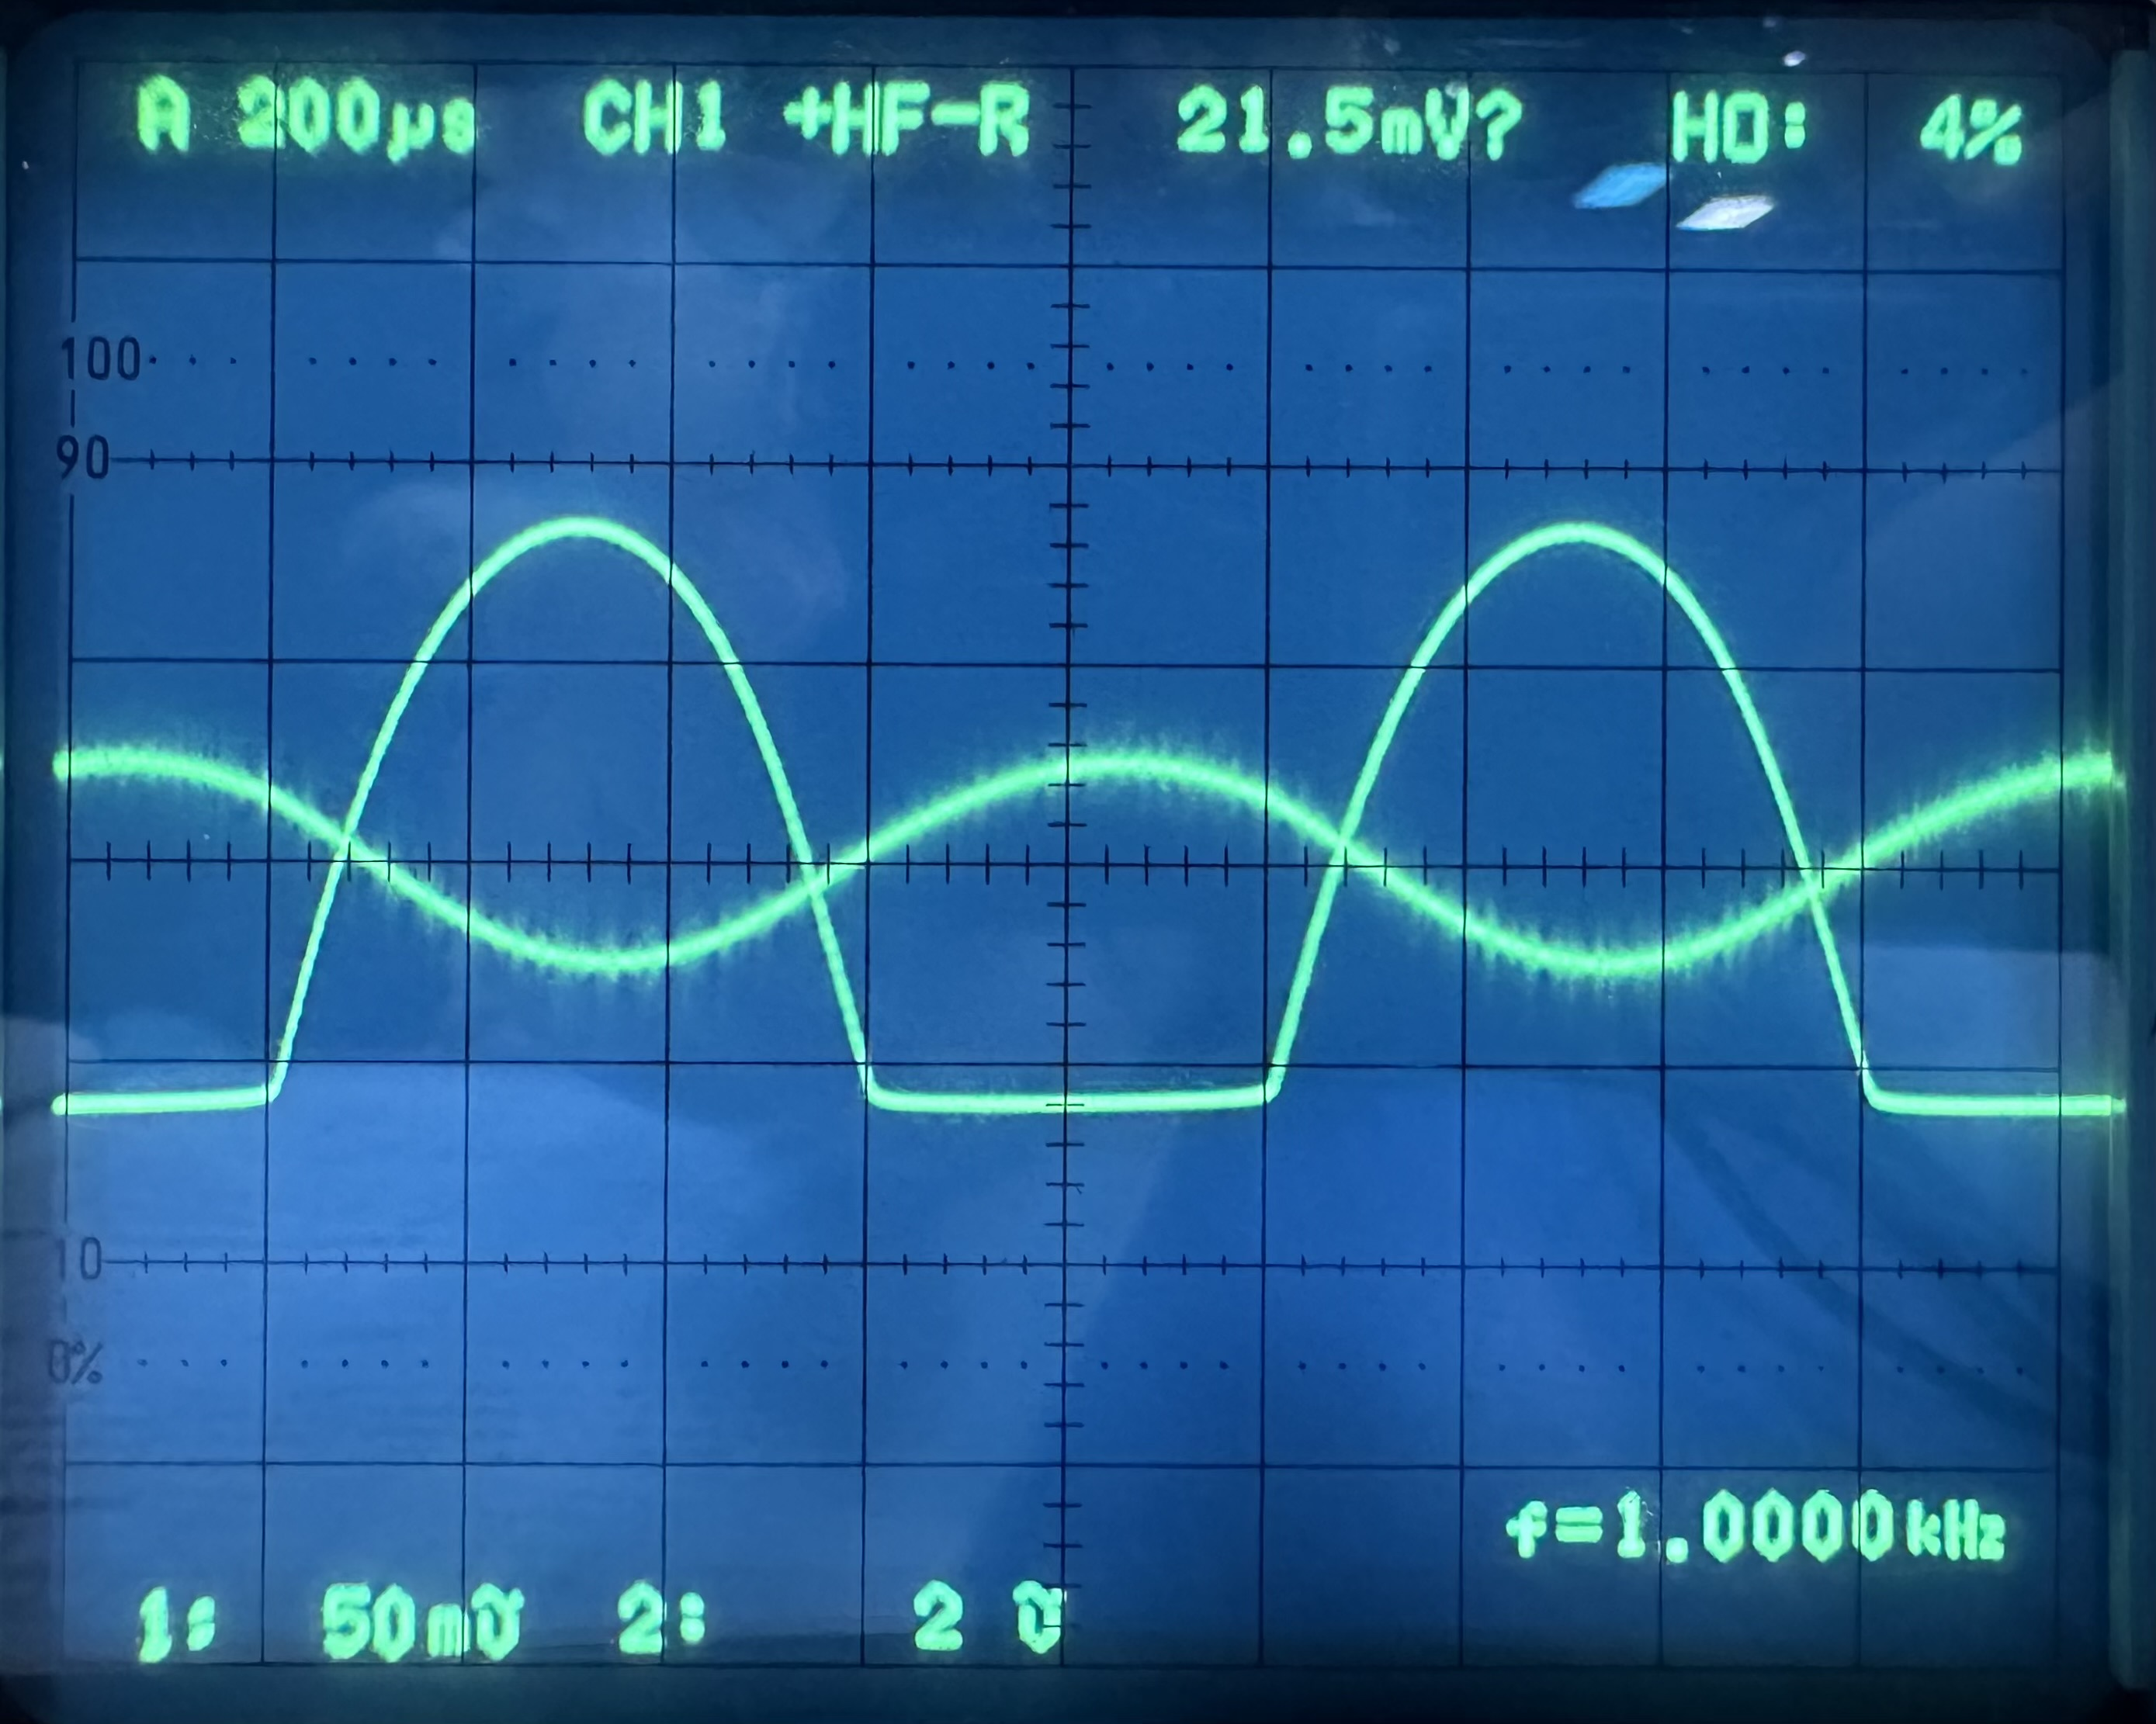
\includegraphics[height=110pt]{BD}}\\
        {\small 图九:输出波形图像}
    \end{figure*}

    \subsection{注意事项}\label{subsec:20}
    {{在记录静态工作点各测量值时,要使输入信号短路(即$u_i=0$)。}}
    {{在记录电位器$R_W$值时,要使$R_W$与电路断开,没有电流流过。}}
    \vspace{1cm}


    \section{思考题}\label{sec:8}

    \subsection{加入输入信号时,输出波形会出现哪几种失真?分别是什么原因引起的?}\label{subsec:q1}

    \subsection{调整静态工作点时,$R_{B2}$是$10k$电阻与电位器$R_W$相串联,而不能直接用电位器,为什么?}\label{subsec:q2}

    \subsection{对于本次的单管放大电路,实现放大的条件是?}\label{subsec:q3}
    \vspace{1cm}


    \section{实验总结}\label{sec:9}
    {{本次实验学习了共射极单管放大器静态工作点的测量与调试方法, 实践了放大电路的交流特性等性能指标的测量方法,
    加深了对放大器各种动态指标的理解,掌握了静态工作点与输出波形失真的关系。
    促进了对单管放大器的理解,有利于线性电子线路课程的学习。}}
    \vspace{1cm}

    \bibliography{main}
    \bibliographystyle{plain}

\end{document}
